The following are the results of applying our approach to both small-scale and large-scale data, with small-scale referring to the 16 sorting and searching program samples from GeeksForGeeks (with an end-goal to differentiate sorting and searching programs), while the large-scale also includes the data files from ByteWeight, which consist of a variety of binutils programs compiled using different compilers and different compiler arguments.

\subsection{Small-Scale Results}

Below are the results of small-scale experiments with LDA and hLDA, both of which perform quite well.

\subsubsection{LDA Results}

\begin{figure}
  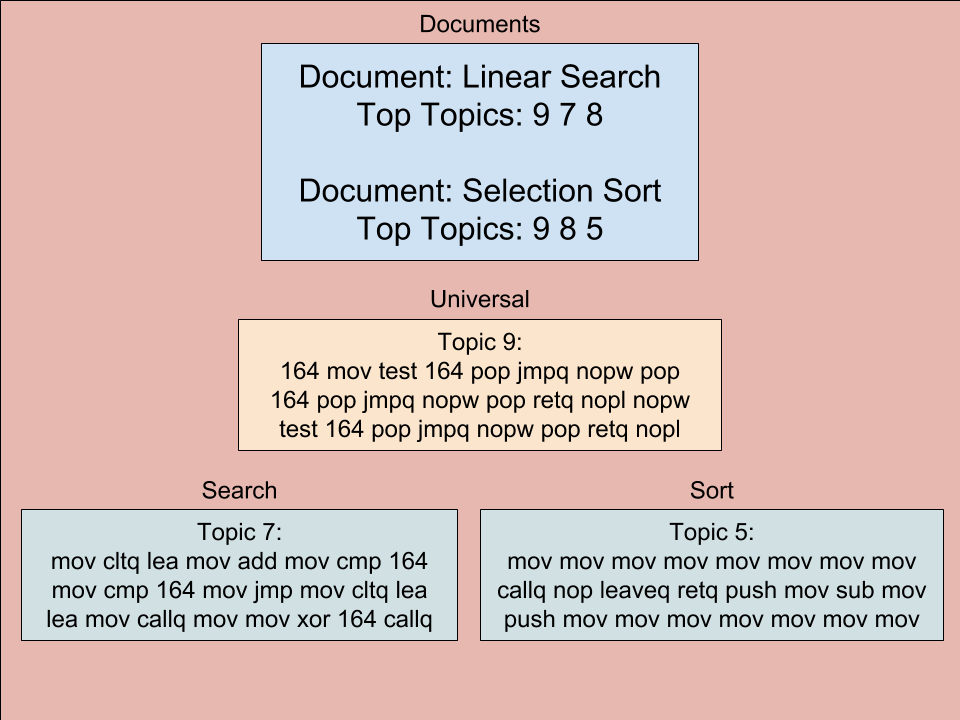
\includegraphics[width=\linewidth]{./figures/ss_fig.png}
  \caption{Side-by-side comparison of Linear Search and Selection Sort. Selection sort can be thought to contain the entirety of linear search (as a slightly modified linear search is used in the selection sort algorithm), so these two programs will be the most similar while still having different purposes.}
  \label{fig:small_lda}
\end{figure}

\begin{table}[]
\centering
\caption{Final results of small-scale LDA model. The top topics are determined based on the learned document-topic distribution. Focus on specific topics is contained in Figure \ref{fig:small_lda}. Hyperparameters for these results were the following: Number of topics = 13, $\alpha = 1e-10, \beta = 0.1$}
$\begin{array}{		l	l	l	l	}
\multicolumn{4}{c}{$LDA Table Results$}                  \\ \hline
$Program$                & \multicolumn{3}{c}{$Top Topics$} \\ \hline
Binary Search          & 9        & 7         & 12       \\ \hline
Interpolation Search   & 9        & 2         & 7        \\ \hline
Linear Search          & 9        & 7         & 8        \\ \hline
Rec. Linear Search     & 9        & 11        & 12       \\ \hline
Jump Search            & 9        & 11        & 19       \\ \hline
Exponential Search     & 9        & 7         & 12       \\ \hline
Bubble Sort            & 9        & 8         & 5        \\ \hline
Rec. Bubble Sort       & 9        & 8         & 5        \\ \hline
Merge Sort             & 6        & 9         & 0        \\ \hline
Rec. Merge Sort        & 6        & 9         & 0        \\ \hline
Quick Sort             & 5        & 9         & 11       \\ \hline
Rec. Quick Sort        & 9        & 5         & 8        \\ \hline
Insertion Sort         & 9        & 4         & 8        \\ \hline
Rec. Insertion Sort       & 9        & 4         & 11       \\ \hline
Selection Sort         & 9        & 8         & 5        \\ \hline
Rec. Heap Sort         & 9        & 1         & 11       \\ \hline
\end{array}$
\label{tab:small_lda_tab}
\end{table}

Figure \ref{fig:small_lda} shows a comparison between the Linear Search and Selection Sort programs with n-grams of size 8. The three topics displayed below were the most significant topics. Topic 9 was held as the most heavily weighted topic for most of the programs, and was the second most significant for three of the sixteen. Topics 7 and 5 were found to be the key differentiators between sorting and searching programs, with topic 7 being found in the majority of searching programs and no sorting programs, and topic 5 being found in many sorting programs and no searching programs. The full small-scale results are shown in Table \ref{tab:small_lda_tab}. Note the fact that topic 5 contains indications of heavy data modification (through the large number of mov statements), while topic 7 makes note of array comparisons in a loop.

\subsubsection{hLDA Results}

\begin{table}[]
\centering
\caption{Final results of small-scale hLDA model. Each document is a leaf node in a hierarchy of topics, so those at the same leaf node are most similar. Hyperparameters for these results were the following: Number of levels = 3, number of samples = 500, $\alpha = 10, \gamma = 1, \beta = 0.1$}
$\begin{array}{	l	c	}
\multicolumn{2}{c}{$hLDA Table Results$}                  \\ \hline
$Program$                & $Deepest Topic in Hierarchy$ \\ \hline
Binary Search          & 8       \\ \hline
Interpolation Search   & 8        \\ \hline
Linear Search          & 8        \\ \hline
Rec. Linear Search     & 8       \\ \hline
Jump Search            & 8       \\ \hline
Exponential Search     & 8       \\ \hline
Merge Sort             & 4       \\ \hline
Rec. Merge Sort        & 4        \\ \hline
Bubble Sort            & 10       \\ \hline
Rec. Bubble Sort       & 10        \\ \hline
Quick Sort             & 10       \\ \hline
Rec. Quick Sort        & 10        \\ \hline
Selection Sort         & 10        \\ \hline
Insertion Sort         & 6        \\ \hline
Rec. Insertion Sort       & 6      \\ \hline
Rec. Heap Sort         & 6       \\ \hline
\end{array}$
\label{tab:small_hlda_tab}
\end{table}

Table \ref{tab:small_hlda_tab} shows the final topics corresponding to each of the programs from hLDA. One can observe that all search programs were successfully isolated from all sort programs. In addition, various recursive versions of programs were matched with their non-recursive versions. These results are very promising and clearly indicate tremendous potential for this approach.

\subsection{Large-Scale Results}

This section discusses the results of the large-scale LDA experiments.

\begin{figure}
  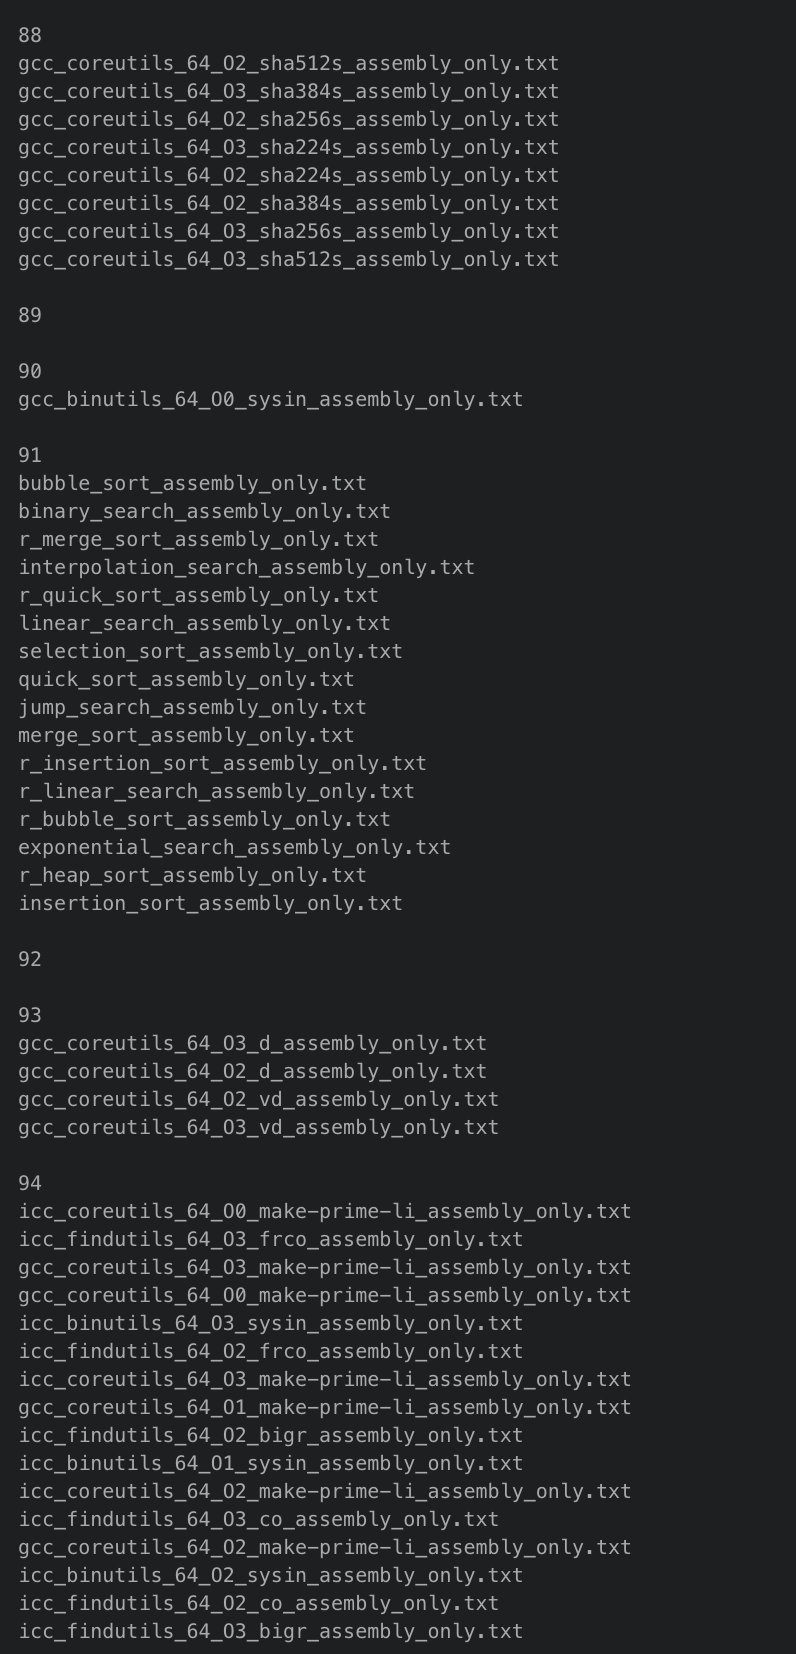
\includegraphics[width=\linewidth]{./figures/large_lda_top_level.png}
  \caption{Documents placed into bins corresponding to their highest-weighted topic. All sorting and searching programs are placed into the same bin, with no other programs being placed within it.}
  \label{fig:large_lda}
\end{figure}

\begin{table}[]
\centering
\caption{Final results of large-scale LDA model. The top topics are determined based on the learned document-topic distribution.  Hyperparameters for these results were the following: Number of topics = 100, $\alpha = 0.001, \beta = 0.001$. The - symbol means that no additional topics were formed as part of its weighting (due to their weights being too small).}
$\begin{array}{	l	l	l	l	l	l	}
\multicolumn{6}{c}{$LDA Table Results$}                  \\ \hline
$Program $               & \multicolumn{5}{c}{$Top Topics$} \\ \hline
Binary  Search          & 91        & 86         & 62 & 78 & 42       \\ \hline
Interpolation  Search   & 91        & 88         & 86 & 61 & 90        \\ \hline
Linear  Search          & 91        & 86         & 33 & 78 &  -      \\ \hline
Rec.  Linear  Search     & 91        & 61        & 86 & 89 & 20       \\ \hline
Jump  Search            & 91        & 78        & 86 & 89 & 27       \\ \hline
Exponential  Search     & 91        & 61         & 86 & 78 & 3       \\ \hline
Bubble  Sort            & 91        & 86         & 51 & 3 & -        \\ \hline
Rec.  Bubble  Sort       & 91        & 86         & 51 & 90 & 80        \\ \hline
Merge  Sort             & 91        & 86         & 61 & 74 & 20        \\ \hline
Rec.  Merge  Sort        & 91        & 86         & 61 & 74 & 20        \\ \hline
Quick  Sort             & 91        & 61         & 86 & 62 & -     \\ \hline
Rec.  Quick  Sort        & 91        & 61         & 86 & 62 & 24        \\ \hline
Insertion  Sort         & 91        & 86         & - & - & -        \\ \hline
Rec.  Insertion  Sort       & 91        & 86         & 61 & - & -       \\ \hline
Selection  Sort         & 91        & 86         & 61 & 80 & 90        \\ \hline
Rec.  Heap  Sort         & 91        & 86         & 61 & 20 & 56       \\ \hline
\end{array}$
\label{tab:large_lda_tab}
\end{table}

Figure \ref{fig:large_lda} shows a small subset of the large-scale results, namely the documents being sorted into bins based on what each document's highest-weighted topic was. As can be seen, all sorting and searching programs are placed in the same bin, with no other programs being placed with them. Additionally, examination of nearby bins reveals other successes, such as isolation of multiple types of hash functions, or different compiled versions of the same program (make-prime-li).

Table \ref{tab:large_lda_tab} details the results of the large-scale test for the original sorting and searching programs. The main difference of this test is to see what topics would be found when there are a wider variety of programs, and how the programs would relate to one another when scaling up. Results show programs pairing with their recursive versions somewhat less frequently, and there do not exist any major differentiators between the sorting and searching programs. That being said, all of the small-scale programs (sorting and searching programs of similar style and the same origin, compiler, and compiler arguments) were found to have the same most significant topic (topic 91). While not as strong as the small-scale results, they are still quite promising.